%%%%%%%%%%%%%%%%%%%%%%%%%%%%%%%%%%%%%%%%%%%%%%%%%%%%%%%%%%%%%%%%%%%%%%%%%%%%%%%%%%%%%%%%%%%%%%%%%%%%%%
% Plantilla básica de Latex en Español.
%
% Autor: Andrés Herrera Poyatos (https://github.com/andreshp) 
%
% Es una plantilla básica para redactar documentos. Utiliza el paquete fancyhdr para darle un
% estilo moderno pero serio.
%
% La plantilla se encuentra adaptada al español.
%
%%%%%%%%%%%%%%%%%%%%%%%%%%%%%%%%%%%%%%%%%%%%%%%%%%%%%%%%%%%%%%%%%%%%%%%%%%%%%%%%%%%%%%%%%%%%%%%%%%%%%%

%-----------------------------------------------------------------------------------------------------
%	INCLUSIÓN DE PAQUETES BÁSICOS
%-----------------------------------------------------------------------------------------------------

\documentclass{article}

\usepackage{lipsum}                     % Texto dummy. Quitar en el documento final.

%-----------------------------------------------------------------------------------------------------
%	SELECCIÓN DEL LENGUAJE
%-----------------------------------------------------------------------------------------------------

% Paquetes para adaptar Látex al Español:
\usepackage[spanish,es-noquoting, es-tabla, es-lcroman]{babel} % Cambia 
\usepackage[utf8]{inputenc}                                    % Permite los acentos.
\selectlanguage{spanish}                                       % Selecciono como lenguaje el Español.

%-----------------------------------------------------------------------------------------------------
%	SELECCIÓN DE LA FUENTE
%-----------------------------------------------------------------------------------------------------

% Fuente utilizada.
\usepackage{courier}
\usepackage{microtype}                  % Mejora la letra final de cara al lector.

%-----------------------------------------------------------------------------------------------------
%	ESTILO DE PÁGINA
%-----------------------------------------------------------------------------------------------------

% Paquetes para el diseño de página:
\usepackage{fancyhdr}               % Utilizado para hacer títulos propios.
\usepackage{lastpage}               % Referencia a la última página. Utilizado para el pie de página.
\usepackage{extramarks}             % Marcas extras. Utilizado en pie de página y cabecera.
\usepackage[parfill]{parskip}       % Crea una nueva línea entre párrafos.
\usepackage{geometry}               % Asigna la "geometría" de las páginas.

% Se elige el estilo fancy y márgenes de 3 centímetros.
\pagestyle{fancy}
\geometry{left=3cm,right=3cm,top=2.5cm,bottom=2.5cm,headheight=1cm,headsep=0.5cm} % Márgenes y cabecera.
% Se limpia la cabecera y el pie de página para poder rehacerlos luego.
\fancyhf{}

% Espacios en el documento:
\linespread{1}                        % Espacio entre líneas.
\setlength\parindent{0pt}               % Selecciona la indentación para cada inicio de párrafo.

% Cabecera del documento. Se ajusta la línea de la cabecera.
\renewcommand\headrule{
	\begin{minipage}{1\textwidth}
	    \hrule width \hsize 
	\end{minipage}
}

% Texto de la cabecera:
\lhead{\subject}               % Parte izquierda.
\chead{}                       % Centro.
\rhead{\doctitle}              % Parte derecha.

% Pie de página del documento. Se ajusta la línea del pie de página.
\renewcommand\footrule{                                 
\begin{minipage}{1\textwidth}
    \hrule width \hsize   
\end{minipage}\par
}

\lfoot{}                                                 % Parte izquierda.
\cfoot{}                                                 % Centro.
\rfoot{Página\ \thepage\ de\ \protect\pageref{LastPage}} % Parte derecha.

%-----------------------------------------------------------------------------------------------------
%	IMÁGENES
%-----------------------------------------------------------------------------------------------------

\usepackage{graphicx}                  % Utilizado para insertar gráficos.
\usepackage{caption}                   % Títulos y leyendas para los gráficos.
\usepackage{subcaption}                % Subfiguras.

%-----------------------------------------------------------------------------------------------------
%	BIBLIOGRAFÍA
%-----------------------------------------------------------------------------------------------------

\usepackage[backend=bibtex]{biblatex}
\usepackage{csquotes}

\addbibresource{references.bib}

%-----------------------------------------------------------------------------------------------------
%	PORTADA
%-----------------------------------------------------------------------------------------------------

% Elija uno de los siguientes formatos.
% No olvide incluir los archivos .sty asociados en el directorio del documento.
%\usepackage{title1}
\usepackage{title2}
%\usepackage{title3}

%-----------------------------------------------------------------------------------------------------
%	TÍTULO, AUTOR Y OTROS DATOS DEL DOCUMENTO
%-----------------------------------------------------------------------------------------------------

% Título del documento.
\newcommand{\doctitle}{Big Data y TPCx-HS}
% Subtítulo.
\newcommand{\docsubtitle}{}
% Fecha.
\newcommand{\docdate}{28 \ de \ Marzo \ de \ 2015}
% Asignatura.
\newcommand{\subject}{Ingeniería de Servidores}
% Autor.
\newcommand{\docauthor}{}
\newcommand{\docaddress}{}
\newcommand{\docemail}{}

%-----------------------------------------------------------------------------------------------------
%	RESUMEN
%-----------------------------------------------------------------------------------------------------

% Resumen del documento. Va en la portada.
% Puedes también dejarlo vacío, en cuyo caso no aparece en la portada.
%\newcommand{\docabstract}{}
\newcommand{\docabstract}{En este texto puedes incluir un resumen del documento. Este informa al lector sobre el contenido del texto, indicando el objetivo del mismo y qué se puede aprender de él.}

\begin{document}

\maketitle

%-----------------------------------------------------------------------------------------------------
%	ÍNDICE
%-----------------------------------------------------------------------------------------------------

% Profundidad del Índice:
%\setcounter{tocdepth}{1}

\newpage
\tableofcontents
\newpage

%-----------------------------------------------------------------------------------------------------
%	SECCIÓN 1: INTRODUCCIÓN
%-----------------------------------------------------------------------------------------------------

\section{Introducción a Big Data}

	Desde hace miles de siglos el ser humano ha investigado la manera de almacenar y recopilar información. Durante muchos siglos la escritura y la pintura eran los únicos mecanismos existentes. Posteriormente surgió la fotografía, los discos de vinilo... Sin embargo, poca información seguía ocupando mucho volumen físico. Gracias a los avances tecnológicos de las últimos décadas, hoy en día disponemos dispositivos electrónicos para el almacenamiento de datos binarios. Además, la evolución de estos dispositivos ha sido frenética. IBM comercializó el primer disco duro en 1956. Este constaba solamente de 5 Mega Bytes de capacidad \cite{hard-disks} mientras que actualmente podemos utilizar discos duros con más de 1 Tera Byte.

	La evolución en la capacidad de cómputo y procesamiento de los computadores también ha sido exponencial. El primer ordenador comercial se presentó en ....(Referencia). Este computador realizaba n cuentas por segundo. Actualmente hablamos de GHz cuando comparamos la velocidad del procesador de un ordenador. Además, es habitual utilizar ordenadores con 8 o más GB de memoria principal. Se han creado benchmarks.... (medio párrafo diciendo para que sirven y que son muy costosos computacionalmente).
	
	Estas nuevas tecnologías han posibilitado que el almacenamiento de datos sea mucho más sencillo. Podemos guardar multitud de archivos multimedia en un dispositivo de unos centímetros y compartirlos con multitud de usuarios. 
	
	El mayor flujo de datos se produce gracias a Internet. Aunque es relativamente joven, se hizo público en 1993, actualmente existen más de mil millones de páginas webs \cite{internet}. Además, multitud de dispositivos electrónicos se conectan e interaccionan con Internet (lo que se denomina Internet de las cosas \cite{big-data-internet-cosas}). Los usuarios de estos dispositivos utilizan aplicaciones web y redes sociales, publicando textos y archivos multimedia. 
	
	Todo este cúmulo de tecnologías y actividades ha dado lugar a que hoy en día haya más de 10 Zeta Bytes de información almacenados (1 ZB = $10^{12}$ GB) (ver la Figura \ref{fig:zeta-bytes}). De hecho, podemos observar que cada año se generan varios Zeta Bytes de información, el crecimiento es exponencial. 5 Exa Bytes ($10^9$ Giga Bytes) se habían almacenado hasta 2003. Actualmente, generamos esta cantidad de información en dos días \cite{big-data}.
	
	 \begin{figure}[h]
	       	\centering
	       	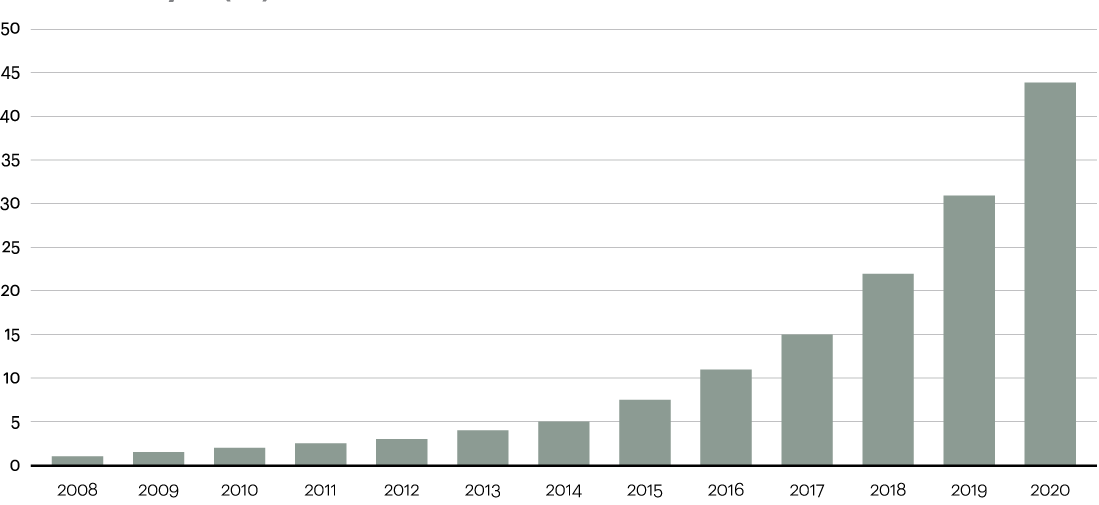
\includegraphics[width=15cm]{./images/Data.png}
	       	\caption{Evolución histórica del número de Zeta Bytes de información almacenados \cite{zeta-bytes}.} 
	       	\label{fig:zeta-bytes}
	 \end{figure}

	Esta cantidad de datos contiene conocimiento. Por ejemplo, todas las empresas almacenan información sobre sus clientes, la actividad y transacciones realizadas. Esta información necesita ser analizada en tiempo real para poder actuar en consecuencia. Aquella empresa que mejor conozca el mercado y actúa rápidamente obtendrá mejores resultados. La ciencia de datos es la rama de la inteligencia artificial que se encarga de tratar y extraer conocimiento de los datos. Se han desarrollado múltiples algoritmos para ello (cita machine learning), que permiten resultados tan impactantes como el reconocimiento de voz o los sistemas de recomendación.
	
	Sin embargo, a pesar de la evolución de los computadores en todas sus facetas, la cantidad de datos e información a procesar y almacenar crece incluso a mayor velocidad. Un ordenador normal no es capaz de tratar tantos GBs de datos. Es más, los algoritmos habituales de aprendizaje necesitan mucho tiempo de cómputo sobre estos conjuntos de datos masivos. Por tanto, necesitamos recurrir a servidores de altas prestaciones y procesamiento distribuido para poder aplicar técnicas de análisis de datos.
	
	Los servidores de altas prestaciones llevan tiempo utilizándose en el ámbito de la inteligencia artificial (referencias). Se han desarrollado herramientas de cómputo en paralelo y distribuido, como OPEN MP y MPI (referencias), que permiten implementar algoritmos distribuidos sobre estos. Sin embargo, estas implementaciones dependen del servidor y son a bajo nivel. Una determinada implementación sobre un esquema hardware puede funcionar bien en determinado momento pero al año tendrá que ser capaz de trabajar con el doble de datos. Esto probablemente suponga la necesidad de ampliar el hardware y rehacer la implementación. Necesitamos pues nuevos paradigma de programación que permitan abstraer el desarrollo de software para plataformas distribuidas del hardware y proporcionen capacidad para el tratamiento de datos masivos.
	
	


	\begin{itemize}
		\item \textbf{Volumen.} El tamaño de la información a procesar es cada vez mayor, por ejemplo, facebook procesa cada día 500 TB de información. Este volumen de datos require técnicas específicas 
		\item \textbf{Velocidad.} Los datos deben ser procesados rápidamente. Normalmente, el procesamiento de los datos debe ser incluso continuo.
		\item \textbf{Variedad.} Los datos a tratar provienen de una gran variedad de fuentes. Por tanto, las herramientas Big Data deben permitir procesar a la vez datos de diferentes características y tamaños.
	\end{itemize}

%-----------------------------------------------------------------------------------------------------
%	SECCIÓN 2
%-----------------------------------------------------------------------------------------------------

\section{Map Reduce}


%-----------------------------------------------------------------------------------------------------
%	SECCIÓN 3
%-----------------------------------------------------------------------------------------------------

\section{Spark y Flink}


%-----------------------------------------------------------------------------------------------------
%	SECCIÓN 4
%-----------------------------------------------------------------------------------------------------

\section{Benchmarks: TPCx-HS}


%-----------------------------------------------------------------------------------------------------
%	SECCIÓN X: REFERENCIAS
%-----------------------------------------------------------------------------------------------------

\section{Referencias}

	\printbibliography

\end{document}